\documentclass[../Práctica.root.tex]{subfiles}
 
\begin{document}

\section{Unidad 1}

\begin{figure}[t]
  \caption{}
  \centering
  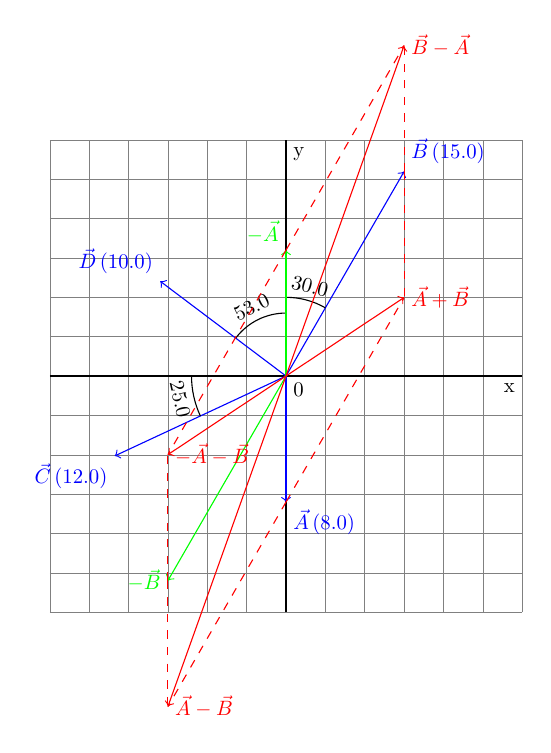
\begin{tikzpicture}[scale=0.2, every node/.style={scale=0.75}]
    \draw[help lines] (-15, -15) grid[step=2.5](15, 15);
    \draw (-15, 0) -- (15, 0) node[anchor=north east]{x};
    \draw (0, -15) -- (0, 15) node[anchor=north west]{y};
    \draw (0, 0) node[anchor=north west]{0};

    \draw[color=blue] [->] (0,0) -- (60:15) node[anchor=south west]{$\vec{B}\left(\SI{15.0}{\meter}\right)$};
    \draw (60:5) arc (60:90:5) node[pos=0.5, anchor=south, sloped]{$\ang{30.0}$};

    \draw[color=blue] [->] (0,0) -- (143:10) node[anchor=south east]{$\vec{D}\left(\SI{10.0}{\meter}\right)$};
    \draw (90:4) arc (90:143:4) node[pos=0.5, anchor=south, sloped]{$\ang{53.0}$};

    \draw[color=blue] [->] (0,0) -- (205:12) node[anchor=north east]{$\vec{C}\left(\SI{12.0}{\meter}\right)$};
    \draw (180:6) arc (180:205:6) node[pos=0.5, anchor=north, sloped]{$\ang{25.0}$};

    \draw[color=blue] [->] (0,0) -- (270:8) node[anchor=north west]{$\vec{A}\left(\SI{8.0}{\meter}\right)$};

    \draw[color=red, dashed] (60:15) -- ++(270:8);
    \draw[color=red, dashed] (270:8) -- ++(60:15);
    \draw[color=red] (270:8) ++(60:15) coordinate(ab) node[anchor=west]{$\vec{A}+\vec{B}$};
    \draw[color=red] [->] (0:0) -- (ab);

    \draw[color=green] [->] (0,0) -- (60:-15) node[anchor=east]{$-\vec{B}$};

    \draw[color=red, dashed] (60:-15) -- ++(270:8);
    \draw[color=red, dashed] (270:8) -- ++(60:-15);
    \draw[color=red] (270:8) ++(60:-15) coordinate(ab) node[anchor=west]{$\vec{A}-\vec{B}$};
    \draw[color=red] [->] (0:0) -- (ab);

    \draw[color=green] [->] (0,0) -- (270:-8) node[anchor=south east]{$-\vec{A}$};

    \draw[color=red, dashed] (60:-15) -- ++(270:-8);
    \draw[color=red, dashed] (270:-8) -- ++(60:-15);
    \draw[color=red] (270:-8) ++(60:-15) coordinate(ab) node[anchor=west]{$-\vec{A}-\vec{B}$};
    \draw[color=red] [->] (0:0) -- (ab);

    \draw[color=red, dashed] (270:-8) -- ++(60:15);
    \draw[color=red, dashed] (60:15) -- ++(270:-8);
    \draw[color=red] (60:15) ++(270:-8) coordinate(ab) node[anchor=west]{$\vec{B}-\vec{A}$};
    \draw[color=red] [->] (0:0) -- (ab);
  \end{tikzpicture}
\end{figure}

\begin{enumerate}
  \item Con los vectores $\vec{A}$ y $\vec{B}$ de la figura 1, use un dibujo a escala para obtener la magnitud y la dirección de:
        \begin{enumerate}
          \item La suma vectorial de $\vec{A}+\vec{B}$ y la diferencia $\vec{A}-\vec{B}$.
                \[
                  \vec{A}+\vec{B} =
                  \begin{bmatrix}
                    \SI{0.0}{\meter} \\
                    \SI{-8.0}{\meter}
                  \end{bmatrix} +
                  \begin{bmatrix}
                    \SI{7.50}{\meter} \\
                    \SI{13.0}{\meter}
                  \end{bmatrix} =
                  \begin{bmatrix}
                    \SI{7.50}{\meter} \\
                    \SI{5.0}{\meter}
                  \end{bmatrix}
                \]
                \[
                  |\vec{A}+\vec{B}| =
                  \sqrt{(\SI{7,50}{\meter})^2+(\SI{5,0}{\meter})^2} =
                  \SI{9,01}{\meter}
                \]
                \[
                  (\vec{A}+\vec{B})_\theta =
                  \arctan{\frac{\SI{5,0}{\meter}}{\SI{7,50}{\meter}}} =
                  \ang{33,7}
                \]

                \[
                  \vec{A}-\vec{B} =
                  \begin{bmatrix}
                    \SI{0.0}{\meter} \\
                    \SI{-8.0}{\meter}
                  \end{bmatrix} -
                  \begin{bmatrix}
                    \SI{7.50}{\meter} \\
                    \SI{13.0}{\meter}
                  \end{bmatrix} =
                  \begin{bmatrix}
                    \SI{-7.50}{\meter} \\
                    \SI{-21.0}{\meter}
                  \end{bmatrix}
                \]
                \[
                  |\vec{A}-\vec{B}| =
                  \sqrt{(\SI{-7,50}{\meter})^2+(\SI{-21,0}{\meter})^2} =
                  \SI{22,3}{\meter}
                \]
                \[
                  (\vec{A}-\vec{B})_\theta =
                  \arctan{\frac{\SI{-21,0}{\meter}}{\SI{-7,50}{\meter}}} =
                  \ang{250}
                \]
          \item Con base en sus respuestas, determine la magnitud y la dirección de: $-\vec{A}-\vec{B}$ y $\vec{B}-\vec{A}$
        \end{enumerate}
  \item Calcule las componentes $x$ e $y$ de los vectores $\vec{A}$,$\vec{B}$,$\vec{C}$ y $\vec{D}$ de la figura 1.
        \[
          \vec{A}_x = \SI{0,0}{\meter}\quad
          \vec{A}_y = \SI{-8,0}{\meter}
        \]
        \[
          \vec{B}_x = \SI{15,0}{\meter}\times\cos{\ang{60,0}} = \SI{7.50}{\meter}\quad
          \vec{B}_y = \SI{15,0}{\meter}\times\sin{\ang{60,0}} = \SI{13.0}{\meter}
        \]
        \[
          \vec{C}_x = \SI{12,0}{\meter}\times\cos{\ang{205,0}} = \SI{-10.9}{\meter}\quad
          \vec{C}_y = \SI{12,0}{\meter}\times\sin{\ang{205,0}} = \SI{-5.07}{\meter}
        \]
        \[
          \vec{D}_x = \SI{10,0}{\meter}\times\cos{\ang{143,0}} = \SI{-7.99}{\meter}\quad
          \vec{D}_y = \SI{10,0}{\meter}\times\sin{\ang{143,0}} = \SI{6.02}{\meter}
        \]
\end{enumerate}
\end{document}
